\subsection*{Problema 11}

\textbf{Enunciado:} \\
Calcular la integral indefinida:
\begin{align*}
I = \int \dfrac{x}{\sqrt{x^2 + 2x + 2}} \, dx
\end{align*}

\textbf{Solución:} \\
Para resolver esta integral, manipulamos el numerador para que aparezca la derivada del radicando, la cual es $2x + 2$. 

Escribimos el numerador como se indica:
\begin{align*}
x = \dfrac{1}{2}(2x + 2) - 1
\end{align*}

Sustituimos esta expresión en la integral original:
\begin{align*}
I &= \int \dfrac{\dfrac{1}{2}(2x + 2) - 1}{\sqrt{x^2 + 2x + 2}} \, dx
\end{align*}

Separamos la integral en dos partes:
\begin{align*}
I &= \dfrac{1}{2} \int \dfrac{2x + 2}{\sqrt{x^2 + 2x + 2}} \, dx \\
&\quad - \int \dfrac{1}{\sqrt{x^2 + 2x + 2}} \, dx
\end{align*}

Definimos $I_1$ para la primera integral y $I_2$ para la segunda, de modo que $I = \dfrac{1}{2}I_1 - I_2$.

Para $I_1$, hacemos el cambio de variable:
\begin{align*}
u &= x^2 + 2x + 2 \\
du &= (2x + 2) \, dx
\end{align*}

Sustituyendo en $I_1$:
\begin{align*}
I_1 &= \int \dfrac{du}{u^{1/2}} = \int u^{-1/2} \, du \\
&= 2u^{1/2} = 2\sqrt{x^2 + 2x + 2}
\end{align*}

Para $I_2$, completamos cuadrados en el denominador:
\begin{align*}
x^2 + 2x + 2 &= (x^2 + 2x + 1) + 1 \\
&= (x + 1)^2 + 1
\end{align*}

La segunda integral se convierte en:
\begin{align*}
I_2 &= \int \dfrac{dx}{\sqrt{(x+1)^2 + 1}}
\end{align*}

Utilizamos la fórmula de integración directa para funciones logarítmicas (o trigonométricas hiperbólicas):
\begin{align*}
I_2 &= \ln \left| (x+1) + \sqrt{(x+1)^2 + 1} \right| \\
&= \ln \left( x + 1 + \sqrt{x^2 + 2x + 2} \right)
\end{align*}

Finalmente, combinamos ambos resultados y agregamos la constante de integración $C$:
\begin{align*}
I &= \dfrac{1}{2} \left( 2\sqrt{x^2 + 2x + 2} \right) \\
&\quad - \ln \left( x + 1 + \sqrt{x^2 + 2x + 2} \right) + C
\end{align*}

Simplificando, obtenemos la solución final:
\begin{align*}
I &= \sqrt{x^2 + 2x + 2} \\
&\quad - \ln \left( x + 1 + \sqrt{x^2 + 2x + 2} \right) + C
\end{align*}

\begin{figure}[H]
	\centering
	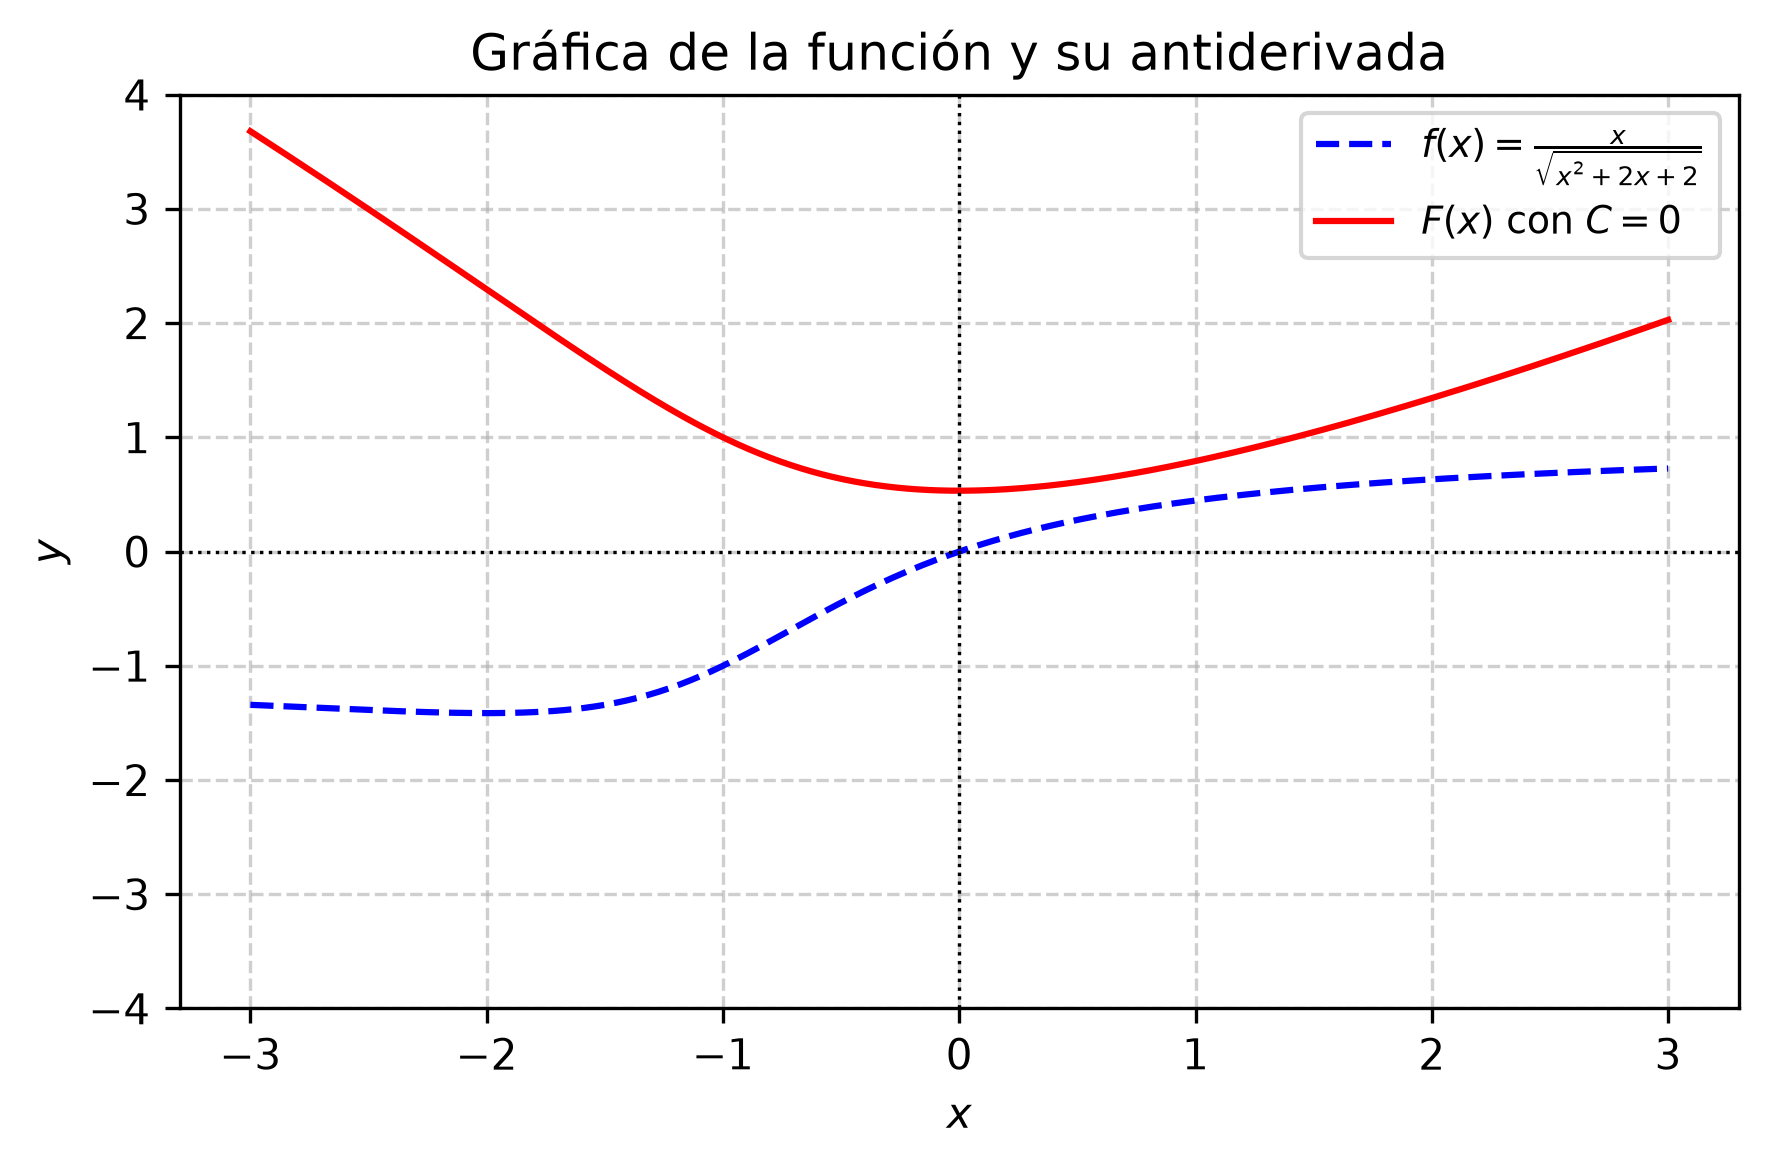
\includegraphics[width=\columnwidth]{semana_05/graficas/SEM05_P11_grafica.png}
	\caption{Representación gráfica de $f(x)$ y su antiderivada $F(x)$ evaluada para la constante de integración $C = 0$ (Problema 11).}
	\label{fig:problema11}
\end{figure}
